\documentclass[a4paper]{article}

\usepackage{cite}
\usepackage[hidelinks]{hyperref}
\usepackage{amsmath}
\usepackage{listings}
\usepackage{xcolor}
\usepackage{pdfpages}
\usepackage{graphicx}
\usepackage{subcaption}

\definecolor{codegreen}{rgb}{0,0.6,0}
\definecolor{codegray}{rgb}{0.5,0.5,0.5}
\definecolor{codepurple}{rgb}{0.58,0,0.82}
\definecolor{backcolour}{rgb}{0.95,0.95,0.92}

\lstdefinestyle{mystyle}{
  backgroundcolor=\color{backcolour},
  commentstyle=\color{codegreen},
  keywordstyle=\color{magenta},
  numberstyle=\tiny\color{codegray},
  stringstyle=\color{codepurple},
  basicstyle=\ttfamily\footnotesize,
  breakatwhitespace=false,
  breaklines=true,
  captionpos=b,
  keepspaces=true,
  numbers=left,
  numbersep=5pt,
  showspaces=false,
  showstringspaces=false,
  showtabs=false,
  tabsize=2
}

\lstset{style=mystyle}

\title{Improving on the ENCODE ChIP-seq normalization pipeline}
\author{Joshua Kim\thanks{joshua.kim@fu-berlin.de}\\EMBL-EBI Hinxton, UK}

\begin{document}
  \maketitle
  \newpage
  \tableofcontents
  \newpage
  \section{Summary}
  This report summarizes the three months I spent at EMBL-EBI in Hinxton, UK, where the primary focus of my work was
  designing a more efficient implementation of the ENCODE ChIP-seq signal normalization pipeline, known as
  align2rawsignal \cite{hoffman_integrative_2013}. In short, align2rawsignal is a tool written by Anshul Kundaje used to
  normalize data generated from ChIP-seq based on a variety of criteria, including mappability of the genome, sequencing depth,
  and replicates. Further, the signal track generated differentiates between regions in the sequence which have no
  read coverage (denoted by a $0$ signal value), and regions which have no signal due because they lie in unmappable areas
  in the genome (denoted by a $NaN$ signal value). It additionally requires mappability tracks generated from a tool
  called Umap \cite{karimzadeh_umap_2018} which generates binary mappabilities for a given read length and reference genome. I was able to
  create a more efficient pipeline, replacing Umap with GenMap \cite{pockrandt_genmap:_2019} and re-implementing align2rawsignal with
  WiggleTools \cite{zerbino_wiggletools:_2014}. In order to better understand the motivation behind this pipeline, I will first briefly explain the
  biological context, and then give an in depth analysis of the pre-existing pipeline before I show my results.

  \section{Background}

    \subsection{DNA, chromatin, and histone modifications}
    DNA is normally organized into beads, known as chromatin, around histone proteins in the nucleus. When in this form,
    regions of the DNA can become more or less transcriptionally available through processes known as histone modifications.
    Acetylation and methylation (addition of acetyl and methyl groups resp.) are the most common forms of modifications, and
    the combination of where the histone is modified and which group is added determines whether the DNA in that chromatin
    will be more or less active. In addition to histones, there are other proteins which can bind to the DNA and affect
    gene transcription. One large family of these are known as transcription factors. Often, knowing where a transcription
    factor binds is an important insight in gene regulation. This can be accomplished in a few ways, but the most common
    is known as ChIP-seq, which combines chromatin immunoprecipitation with high throughput sequencing.
    However, it is not always enough to know where a specific protein binds. One may wish to probe
    more generally at the DNA structure, looking for all accessible regions of the genome. This can be accomplished by
    techniques such as ATAC-seq and DNase-seq, which use different isolation methods to separate and sequence the open regions of DNA.

    \subsection{ChIP-seq, ATAC-seq, and more}
    ChIP-seq \cite{johnson_genome-wide_2007} is a widely used epigenetic technique to identify regions of interest for a given protein. Primarily used
    with transcription factors, it can be split into two subprocesses: chromatin immunoprecipitation followed by high
    throughput sequencing. Chromatin immunoprecipitation is further divided into four steps. First, the DNA and the protein
    of interest are crosslinked reversibly, via UV light or formaldehyde. Then, the DNA is fragmented into lengths of 200-400
    base pairs using either lysates or sonication. Third, the fragments which contain crosslinked DNA-protein pairs are
    precipitated out using antibodies to the protein of interest. Finally, the crosslinking is undone and the proteins
    are digested, while the DNA continues to be purified and sequenced \cite{collas_current_2010}. Once purified, the DNA is then sequenced.
    The key information with the sequencing step is that the entire fragment is often not sequenced. From a 300 base pair
    fragment, it is possible, and common, that only 75-100 base pairs from either end will be sequenced. Thus, instead
    of seeing reads aligning to where the fragment lies in the genome, you will see reads aligning to the start and end
    of the fragment, with the center of the fragment lacking coverage.

    ATAC-seq and DNase-seq are two other common techniques. They are similar to one another in that they probe the entire
    genome looking for open regions, or regions potentially accessible by proteins. However, ATAC-seq is much more relevant
    as it requires significantly less time and significantly fewer cells \cite{buenrostro_transposition_2013}. The difference between these techniques
    and ChIP-seq is that these show all available locations in the genome, whereas ChIP-seq will show all locations which
    a specific protein has bound to.

    Despite the different use cases for the aforementioned techniques, the resulting data is strikingly similar.
    They all submit fragments of length 200 or more to be sequenced, resulting in two peaks around the actual fragments
    when looking at the coverage tracks. Furthermore, the core goal of all of these is the same, to identify regions
    of interest on the genome by looking at differences in sequencing depth. Thus, for the sake of this report I will just
    refer to ChIP-seq, but keep in mind that what I say is applicable to more than just ChIP-seq.

    \subsection{Mappability}
    One final important concept is the mappability of a genome. Mappability is defined as a measure of how often a
    specific sequence with length $k$ occurs in the given genome. If the sequence is unique, it is given a mappability
    of $1$, and this value approaches $0$ the more frequently the sequence occurs in the genome. Thus, for a given $k$ and genome,
    one can iterate through the entire genome base by base, and determine the mappability value of the $k$-mer at each
    position. From there, one could obtain a binary mappability track by only keeping positions with values of $1$, or
    completely unique positions, and setting all other values less than $1$ to $0$. Knowing the mappability of a genome
    can be useful for e.g. preprocessing a fasta file to select only mappable reads.

    In this application, the mappability will be used in two ways. The first way will be in the fragment length calculations,
    where the mappability is used to filter the coverage values to regions that are completely mappable. This improves
    the accuracy of the fragment length calculation primarily by reducing noise and bias. Ramachandran, et. al showed
    that differences in mappability can introduce an artificial bias into the fragment length calculation, and by masking
    the reads for mappability, this bias can be corrected for \cite{ramachandran_masc:_2013}. The second usage of the mappability is at the
    normalization step, where the mappability is used to normalize the signal coverage values. If a one region is a
    highly mappable region, and another region is not, we would expect there to be more reads in the more mappable region.
    Thus, this is normalized for, so that a highly mappable region does not display a peak where it should not be.

  \section{The Old Pipeline}
  Here I will discuss the methods of the previous pipeline, along with any motivation for switching to another pipeline.

    \subsection{Umap}
    Umap is a tool developed originally by Anshul Kundaje. The original script was written in MATLAB, but is no longer
    publicly available. Mehran Karimzadeh then reimplemented Umap using Python in 2016, adding some new features such as
    calculating the mappability of the bisulfite-converted genome \cite{karimzadeh_umap_2018}. Umap in its essence is
    comprised of 3 steps. For a given $k$ value, it will
    \begin{enumerate}
      \item generate all possible $k$-mers,
      \item map each of the $k$-mers to the genome,
      \item and mark all uniquely aligned positions.
    \end{enumerate}
    The step that is problematic is step 2, where the authors use Bowtie \cite{langmead_ultrafast_2009} to align each $k$-mer to the genome.
    While Bowtie is certainly an industry standard, it is better optimized for actually aligning reads to a reference
    sequence, not just aligning $k$-mers to calculate mappability. Thus, the runtime for Umap ends up being approximately
    200 CPU hours on a single core, or 30 minutes on 400 cores.

    Additionally, Umap has soft requirement that it can only run on Sun Grid Engine (SGE) machines. SGE is a cluster
    software similar to SLURM or LSF. However, there is no guarantee that every machine uses SGE, and to convert Umap to
    SLURM or LSF compatible software is tedious and has not yet been publicly done.

    \subsection{align2rawsignal}
    Align2rawsignal is another tool developed by Anshul Kundaje, specifically for analysis of ENCODE data \cite{hoffman_integrative_2013}.
    It is also developed in MATLAB, and requires the MATLAB runtime library to execute. As an input, it requires one or more
    BAM files, along with the fragment length(s) ($L_i$) for each file. It then proceeds as follows:
    \begin{enumerate}
      \item The read starts are shifted in the 3' direction by $\frac{L_i}{2}$ and then coverage is computed per strand.
      \item A weighted sum of read counts is calculated using a Tukey kernel of width $w$, centered at each position $x$.
            This weighted sum $F(x)$ represents the approximate number of sequenced fragments overlapping any position $x$.
      \item The fragment counts from both strands are added together.
      \item Steps 1. through 3. are then repeated for the binary mappability track with the same read length, to generate the
            local cumulative mappability ($M(x)$). $M(x)$ indicates the number of positions around $x$ which can potentially
            contribute read counts based on mappability.
      \item An expected fragment count track is then calculated using the following formula:
      \begin{equation}
        \label{eq:1}
        E(x) = \frac{M(x)*R}{G}
      \end{equation}
      where $R$ is the total number of mapped reads in the input file, and $G$ is the total mappable genome size across both strands.
      \item The normalized signal $S(x)$ is computed using the formula
      \begin{equation}
        \label{eq:2}
        S(x) = F(x) / E(x)
      \end{equation}
      \item Signal values at unmappable regions and at positions where $E(x) <= \frac{max_xE(x)}{4}$ are set to $NaN$, so that
            positions with a value of 0 represent mappable positions where no reads mapped, and positions with no values
            are completely unmappable positions.
    \end{enumerate}
    The end result is a normalized signal track $S(x)$, where at each base position $x$ the signal has been normalized by
    number of reads and mappability. While nothing is inherently wrong with the tool, it is not as efficient as it could be,
    as it reimplements several things which already have efficient implementations, e.g., reading and writing to standard file formats.

  \section{The New Pipeline}
  In the new pipeline, Umap has been replaced by GenMap, and align2rawsignal has been re-written using Python3 and WiggleTools.
  This introduces several benefits, which are detailed below.

    \subsection{GenMap}
    GenMap is a tool written in C++ using the SeqAn library \cite{pockrandt_genmap:_2019}. The principle ideas of GenMap are the same as with Umap:
    to calculate the mappability for a given length $k$ at each position in the genome. However, GenMap is more efficient than
    Umap by several orders of magnitude. This is primarily due to a few intelligent choices made in GenMap:
    \begin{enumerate}
      \item The first choice was to use an EPR dictionary, which is an implementation of a bidirectional FM index.
            This is an alternative to the index used in the Bowtie aligner, which is a unidirectional FM index based on
            the Burrows Wheeler Transform. The benefit of the bidirectional index is that it supports forward \textit{and}
            reverse lookups in constant time. Using this, GenMap can take advantage of similar $k$-mers which share a large
            portion of their content, and only the beginning and end portions are different.
      \item The next choice was the use of optimum search schemes. Optimum search schemes take advantage of a bidirectional
            FM index to split a text into parts. They dictate which parts of the search string should be searched in what order
            to minimize the number of errors allowed in the first pieces of each search, thereby limiting the number of edges
            in the search tree.
      \item Finally, mappability values for redundant $k$-mers are recycled. That is, while computing the mappability of
            a $k$-mer, all occurrences of that $k$-mer in the text will have its mappability value filled in. Then, when
            that position is encountered later on, it can already be skipped.
    \end{enumerate}
    By utilizing these improvements, GenMap is able to achieve a runtime of ~2.5 minutes on
    16 cores, as opposed to 30 minutes on 400 cores with Umap. Additionally, it does not depend on any specific clustering software

    \subsection{WiggleTools}
    WiggleTools is another tool written in C++. There are many different functions included within WiggleTools which are
    used to manipulate and calculate statistics on coverage data. Its main benefit is that it streams in data from input files and then
    immediately performs online calculations and streams its output, requiring very little memory overhead. For comparison,
    align2rawsignal loads chunks of the input files into memory, splitting the file by default into 20 chunks. Additionally,
    WiggleTools doesn't require the MATLAB runtime library, and just requires a default GNU compiler.
    One other advantage WiggleTools provides is its ability to use standard filetypes as input and output formats. It relies on the
    HTSlib and libBigWig libraries, which are standard libraries used for input and output of sequencing data.
    This is crucial because indexed binary files, such as BigWig and BAM files, provide
    significantly quicker access to the data stored in them.

  \section{Methods}

    \subsection{Fragment length estimation}
    The fragment lengths were estimated using pearson correlation values as a measurement:

    \lstinputlisting[language = Python, firstline = 69, lastline = 75]{../scripts/wiggletoolsSigNorm.py}

    The key part of the code is line 4, where \verb$wiggletools pearson$ is called. In this line, the pearson correlation
    values are calculated between the positive and negative strands, where only values in \textit{dual strand mappable}
    regions are used for the calculation. \textit{Dual strand mappability} is defined as regions where a read mapping to
    position $x$ on the positive strand, and position $x + shift$ on the negative strand, are both mappable. This is in contrast
    to the call on line 7, where a naive pearson correlation is calculated without any regard for mappability. The technique
    of filtering to only dual mappable regions is adapted from MaSC \cite{ramachandran_masc:_2013}, and does well to reduce artefacts introduced
    by noise and random data. However, I found that this was not enough, and resulted in the very first points, corresponding
    to the read length of the sample, being artificially inflated.

    Thus, I introduced one final correction technique, where I ignore any max value if it occurs at the very first
    shift value, and then I smooth the entire curve using a moving average filter:
    \lstinputlisting[language = Python, firstline = 88, lastline = 94]{../scripts/wiggletoolsSigNorm.py}
    This is a reasonable assumption to make, as there are two possible scenarios:
    \begin{enumerate}
      \item The max value is always the smallest shift value. This means the trend is a constant negative slope, and
            there is likely some sort of error in the read data.
      \item The max value will eventually jump to another value which is not the left-most shift value. This is much
            more likely to be the true shift value.
    \end{enumerate}
    With this, I had a method to calculate the fragment lengths of any input file. I also managed to parallelize it,
    distributing the pearson correlation calculations among a variable number of input processors.

    \subsection{Normalization}
    \label{methods:normalization}
    The normalization method used was a fairly accurate reimplementation of the original tool by Kundaje \cite{hoffman_integrative_2013}, so
    the details won't be elaborated on here. However, I will highlight two small differences.

    The first is that Kundaje's tool used read start counts in their signal. In my implementation, I used read
    coverage counts. Thus, to obtain an expected fragment count track, I had to multiply the total mapped read count by the read
    length, as such:
    \begin{equation}
      \label{eq:3}
      E(x) = \frac{M(x)*R*RL}{G}
    \end{equation}
    The only difference to equation \ref{eq:1} is the addition of the $RL$ variable, which represents the read length.

    The second difference is that the normalization by Kundaje uses a Tukey kernel to perform an aggregate sum,
    where the central window length is equal to the fragment length with a weight of 1, and then it tapers on both ends
    with the weights following a cosine curve. The entire Tukey kernel window is of length 300. In our normalization,
    we simplify this further and just use a simple windowed sum of length 300.

  \section{Results}
  One key result that I am unable to definitively speak on is efficiency. Although both GenMap and WiggleTools are more
  efficient than their counterparts in theory, I was unable to run practical experiments comparing the two. The main
  reason was that both of them had preset configurations or requirements that I was not able to establish on the
  EMBL-EBI cluster system. For Umap, I was unable to switch it from using the SunGrid Engine to using LSF, and I
  was unable to download and install the MATLAB runtime environment to run align2rawsignal.

    \subsection{Fragment length estimation}
    Figure \ref{fig:1} shows three separate samples to show some preliminary results. Each one was run first with naive perason calculations,
    then with mappability masking, and finally with mappability masking \textit{and} removing the first max values.

    As you can see, the peak shifts significantly from the first row compared with rows 2 and 3. This is due to the
    biased introduced by mappability differences.
    According to Ramachandran, et. al, using the mappability as a mask was enough to completely eliminate the preference
    for the read length. However, I found that there was still a strong tendency to overweight the shift values close to
    the read length. In figure \ref{fig:1}, on row 2, the first sample predicted the correct fragment length. However,
    the following two samples both predicted a length of 76, which corresponds to the read length. Thus, by filtering out
    those max values occurring in the very beginning, and smoothing the data, we can get much more accurate values,
    shown in row 3.

    \subsection{Normalization}

    The normalization results are difficult to display, as they are very large signal track files. The alternative
    assessment used was to generate various statistics on the sample files pre- and post-normalization, including
    area under the curve (AUC), covariance, mean value, and max value.

    % Include plots with statistics.

    One interesting note is that although my implementation
    was very similar to the implementation described in Michael Hoffman's paper \cite{hoffman_integrative_2013}, the
    end results looked a bit different to one another. This can be attributed to a few possibilities.

    One possibility is that the differences mentioned in section \ref{methods:normalization} account for more variability
    in the normalization than anticipated. However, the read length factor in equation \ref{eq:3} should cancel itself out
    within the data, since the data is read coverage and not read start counts.

    Another possibility is that there is an error in align2rawsignal. Looking at figure \ref{fig:2}, you see a comparison
    between track data normalized by align2rawsignal, and track data normalized by my implementation. In the
    supplementary file of \cite{hoffman_integrative_2013}, they explain that the final step of the normalization is to
    discard signal track values which lie in regions of low mappability, or in completely unmappable regions. However,
    the figure clearly displays a region of low/non-mappability where align2rawsignal fails to remove the signal. This
    could be why the AUC is so much higher in align2rawsignal.

    However, despite the differences in the two signal tracks, the overall trends in both sample pools seems to be similar.

  \section{Conclusion}
  In my three months at EMBL-EBI, under supervision of Dr. Daniel Zerbino, I worked on reimplementing the ENCODE ChIP-seq
  normalization pipeline. This pipeline is a widely used series of tools meant to normalize raw ChIP-seq and other
  epigenetic datasets from read coverage to normalized sequenced fragment counts. As a final result, I present my
  reimplementation of the pipeline, primarily focused on using GenMap \cite{pockrandt_genmap:_2019} for the mappability
  track generation, and WiggleTools \cite{zerbino_wiggletools:_2014} for the normalization calculations.

  \section{Future work}
  There are a number of things I would like to continue working on to present a more final product.

  \begin{enumerate}
    \item Establishing a set of rigorous and reliable tests. As I was unable to get Umap and align2rawsignal functioning,
          I would like to work on getting them running so that I can test them against my current implementation.
    \item Extending the pipeline to accept paired end input. Currently, it only functions on single end data. However,
          the extension to paired end data is not too difficult to imagine. With paired end data, the entire fragment
          length estimation can be skipped, as that information can be obtained from the distance between the paired
          end reads. Then, the primary difference is in the normalization of the signal, where the mappability track
          would be different, in order to account for the joint mappability of the primary and secondary reads.
    \item Extending the pipeline to work with replicate samples. This is something that is currently possible in
          align2rawsignal, but not yet possible in my implementation. However, it is fairly trivial to implement, as it
          only affects the normalization step. It is, in essence, just an average of all of the intermediate signal
          tracks generated by each replicate. For example, the expected signal formula would then look as such:
          \begin{equation}
            \label{eq:4}
            E(x) = \frac{M_i(x)*R_i*RL_i}{G}
          \end{equation}
          And the final normalized signal as such:
          \begin{equation}
            \label{eq:5}
            S(x) = \sum_{i \in Replicates}\left(\frac{F_i(x)}{E_i(x)}\right)
          \end{equation}
  \end{enumerate}

  \bibliography{FinalWriteUp}{}
  \bibliographystyle{plain}

  \newpage
  \section{Figures and Plots}

  \begin{figure}[h!]
    \makebox[\textwidth][c]{
    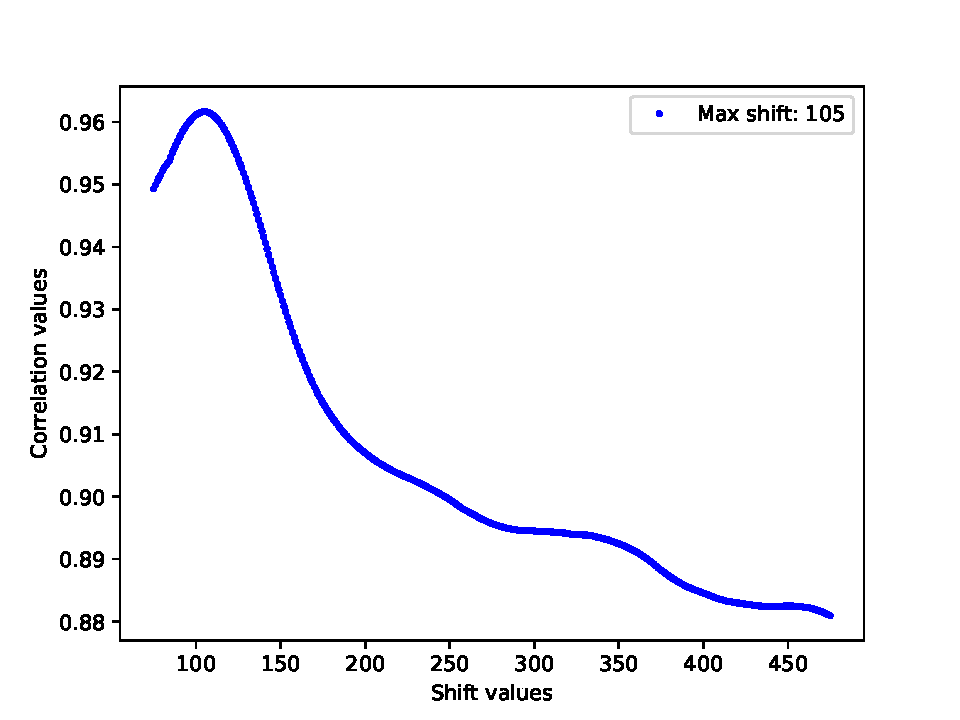
\includegraphics[width = .55\textwidth]{images/FragLength_Naive1}
    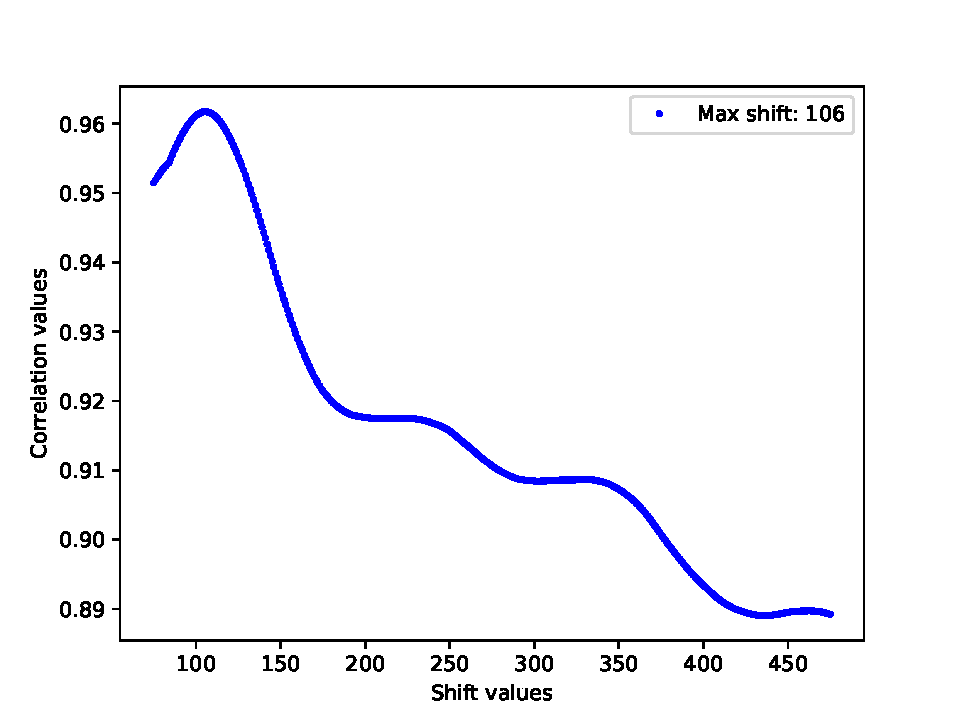
\includegraphics[width = .55\textwidth]{images/FragLength_Naive2}
    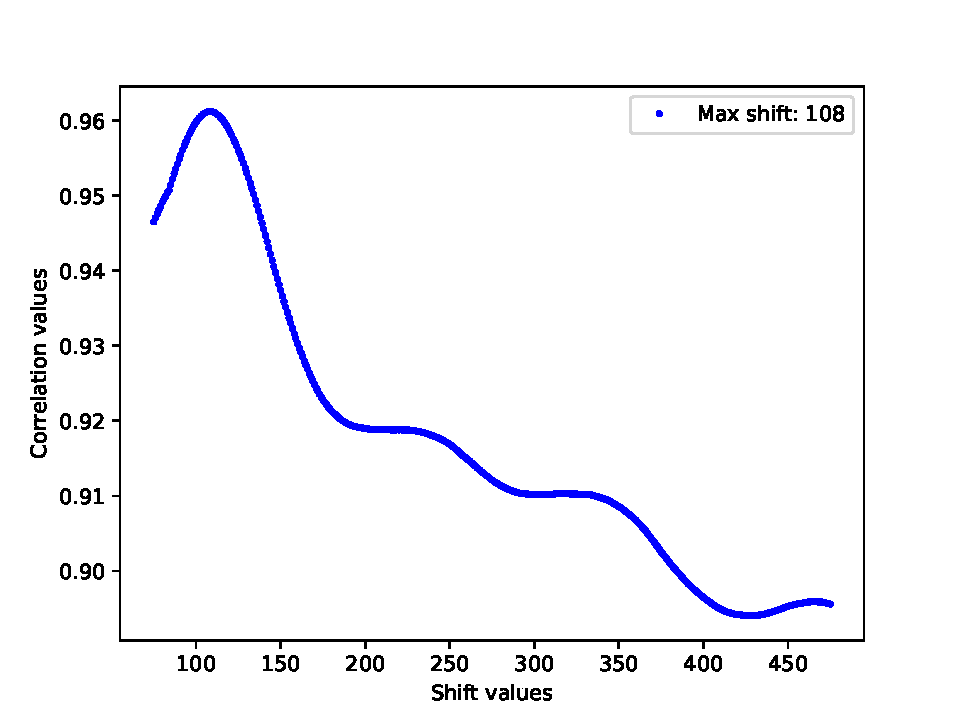
\includegraphics[width = .55\textwidth]{images/FragLength_Naive3}}

    \makebox[\textwidth][c]{
    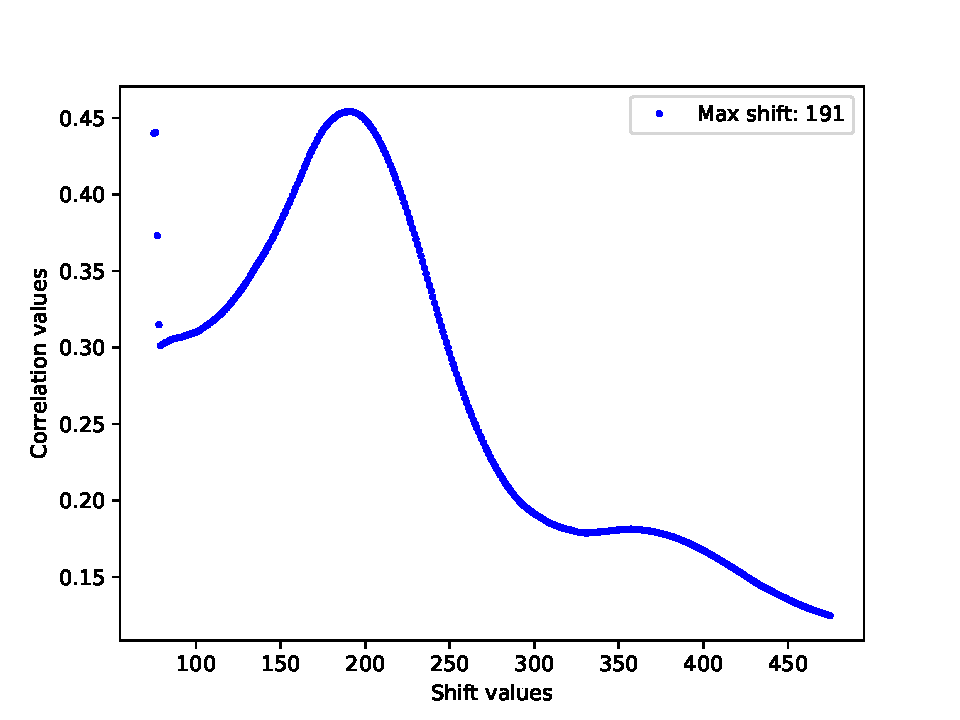
\includegraphics[width = .55\textwidth]{images/FragLength_Mappability1}
    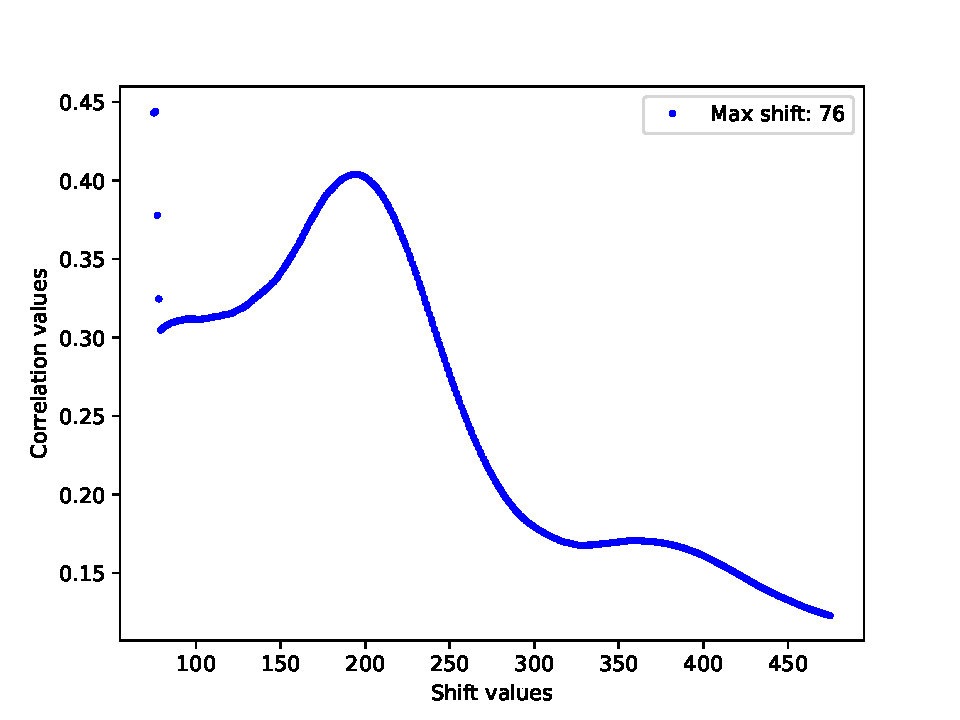
\includegraphics[width = .55\textwidth]{images/FragLength_Mappability2}
    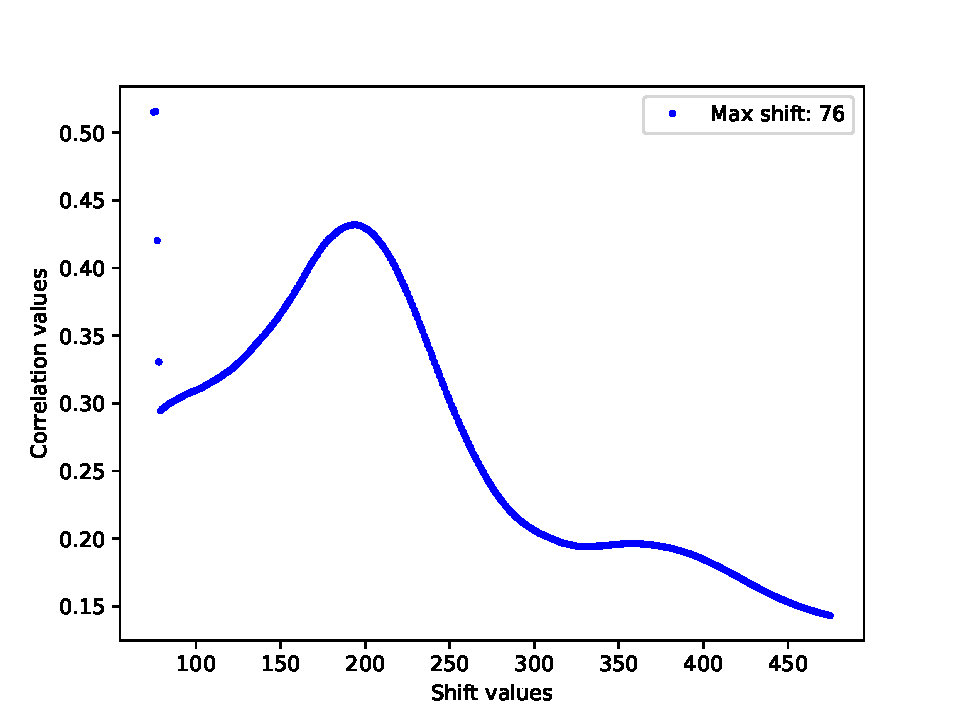
\includegraphics[width = .55\textwidth]{images/FragLength_Mappability3}}

    \makebox[\textwidth][c]{
    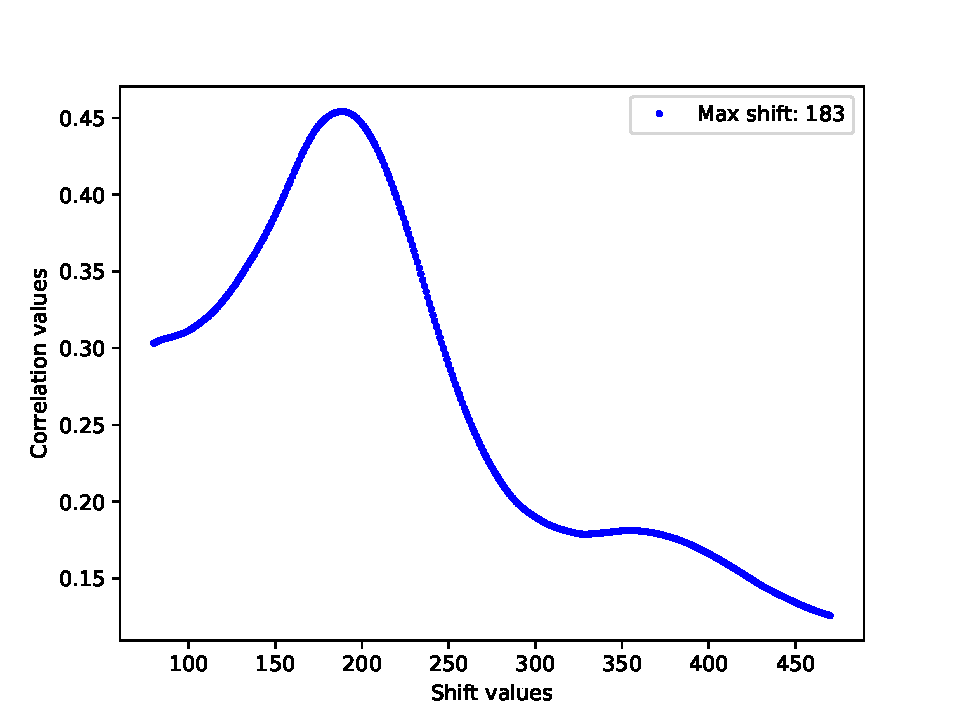
\includegraphics[width = .55\textwidth]{images/FragLength_MapFilter1}
    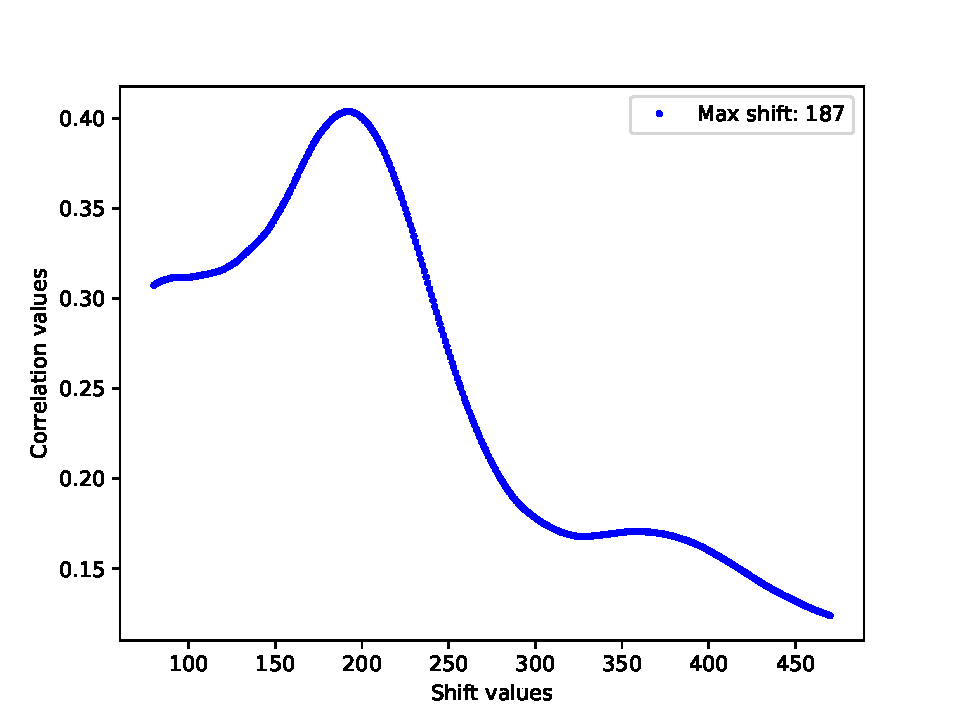
\includegraphics[width = .55\textwidth]{images/FragLength_MapFilter2}
    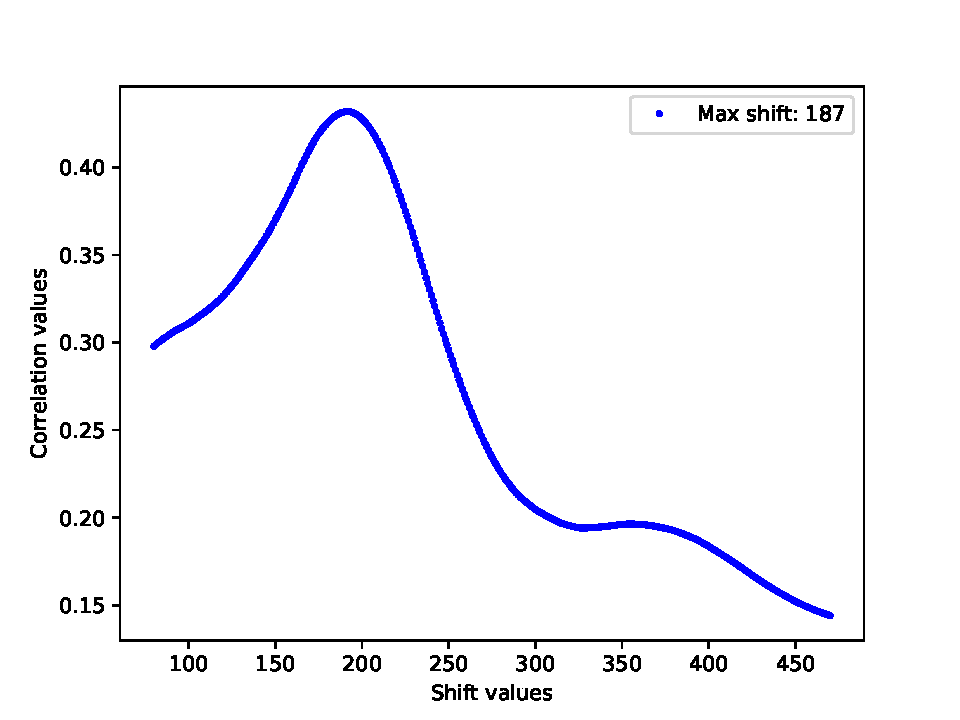
\includegraphics[width = .55\textwidth]{images/FragLength_MapFilter3}}
    \caption{Three samples processed naively (Row 1), using mappability to mask unmappable values (Row 2), and then using mappability and filtering the leftmost max values (Row 3). The max shift values are: (Row 1) 105, 106, 108, (Row 2) 191, 76, 76, (Row 3): 183, 187, 187}
    \label{fig:1}
  \end{figure}

  \begin{figure}[htp]
    \makebox[\textwidth][c]{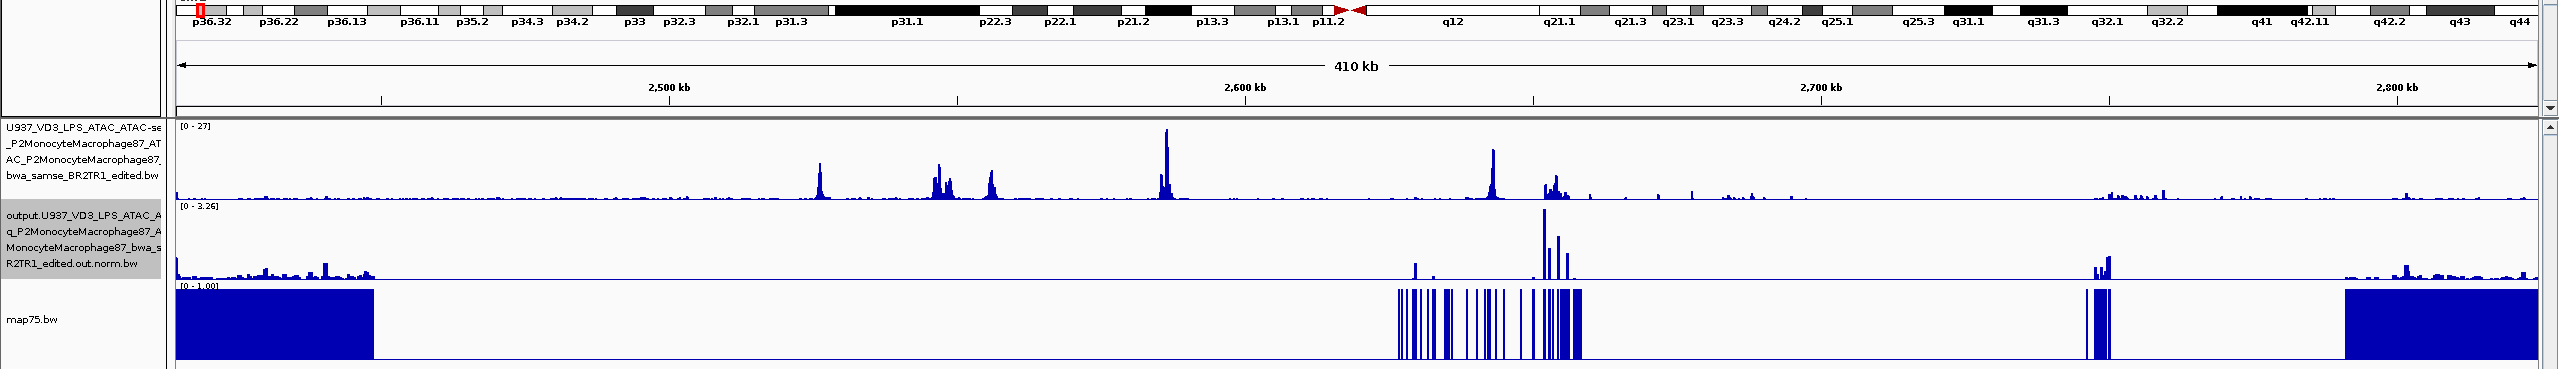
\includegraphics[width = 1.65\textwidth]{images/Unmappable_regions.png}}

    \caption{A comparison between Kundaje's align2rawsignal (track 1) and my reimplementation (track 2), with the mappability in this region displayed in track 3. Note align2rawsignal shows non-zero values in unmappable regions, despite claiming to discard signal in these regions.}
    \label{fig:2}
  \end{figure}
\end{document}
